\documentclass{article}

\usepackage{graphicx}
\usepackage{tikz}
\usepackage{tikzsymbols}
\usetikzlibrary{calc,patterns,shapes.geometric}
\pagestyle{empty}
\usepackage[margin=0pt]{geometry}
\geometry{papersize={14in,12in}}

\def\centerarc[#1](#2)(#3:#4:#5){\draw[#1] ($(#2)+({#5*cos(#3)},{#5*sin(#3)})$) arc (#3:#4:#5);}

\begin{document}
	\begin{figure}
		\centering
		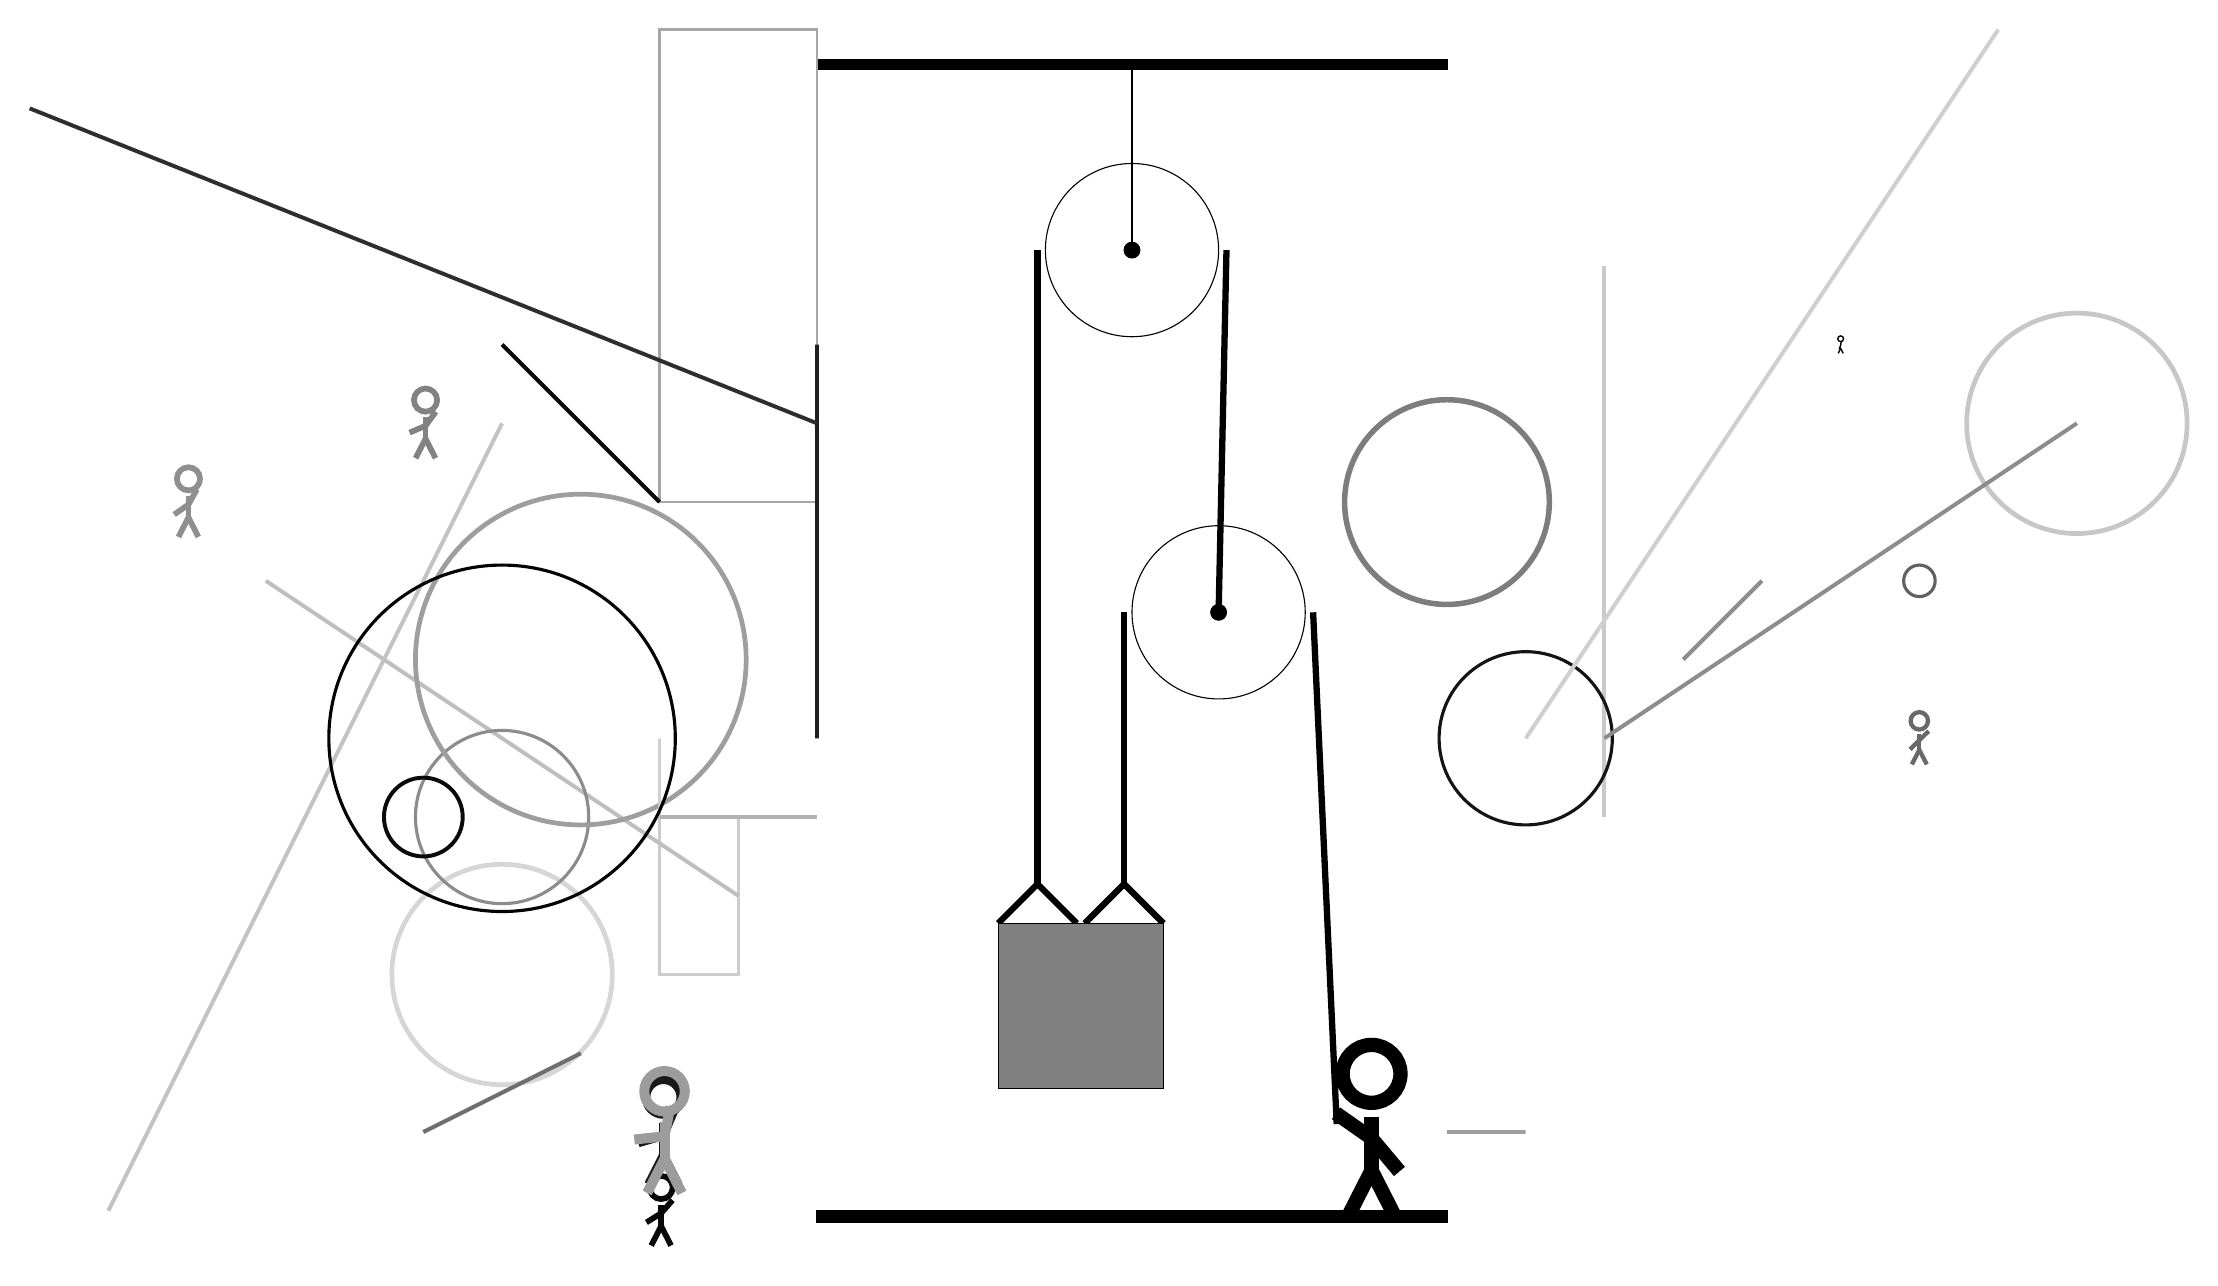
\begin{tikzpicture}
			%%%%% START %%%%%
			
			\draw[fill=black] (-2, 11.5) rectangle (6, 11.625);
			
			\draw (2, 9.2) circle (1.1);
			\draw[fill=black] (2, 9.2) circle (0.1);
			\draw[thick] (2, 9.2) -- (2, 11.5);
			
			\draw[line width=0.4mm, color=black!20] (-4, 0) rectangle (-3, 2);
			
			\draw[line width=0.5mm, color=black!45](9, 4) -- (10, 5);
			\node[line width=0.4mm, color=black!44] at (-10, 6) {\Strichmaxerl[4][35][61]};
			\draw[line width=0.5mm, color=black!25](-3, 1) -- (-9, 5);
			\draw [line width=0.4mm, color=black!62](12, 5) circle (0.2);
			\draw[line width=0.5mm, color=black!24](-6, 7) -- (-11, -3);
			
			\draw[line width=0.5mm, color=black!21](8, 9) -- (8, 2);
			
			\draw[line width=0.3mm, color=black!35] (-2, 12) rectangle (-4, 6);
			\draw [line width=0.6mm, color=black!22](14, 7) circle (1.4);
			\draw [line width=0.6mm, color=black!16](-6, 0) circle (1.4);
			
			\draw[line width=0.6mm, color=black!88] (-2, 3) rectangle (-2, 8);
			
			\draw [line width=0.4mm, color=black!45](-6, 2) circle (1.1);
			\draw[line width=0.5mm, color=black!57](-5, -1) -- (-7, -2);
			
			\node[line width=0.6mm, color=black!49] at (-7, 7) {\Strichmaxerl[4][23][54]};
			\node[line width=0.2mm, color=black!97] at (11, 8) {\Strichmaxerl[1][70][81]};
			\draw [line width=0.6mm, color=black!38](-5, 4) circle (2.1);
			\node[line width=0.4mm, color=black!90] at (-4, -2) {\Strichmaxerl[6][16][67]};
			\draw [line width=0.4mm, color=black!92](7, 3) circle (1.1);
			\node[line width=0.2mm, color=black!59] at (12, 3) {\Strichmaxerl[3][45][44]};
			\draw[line width=0.4mm, color=black!18] (-4, 2) rectangle (-4, 3);
			\draw [line width=0.7mm, color=black!51](6, 6) circle (1.3);
			
			\draw [line width=0.4mm, color=black!99](-6, 3) circle (2.2);
			\draw[line width=0.5mm, color=black!19](7, 3) -- (13, 12);
			\draw [line width=0.5mm, color=black!96](-7, 2) circle (0.5);
			\node[line width=0.3mm, color=black!97] at (-4, -3) {\Strichmaxerl[4][32][49]};
			\draw[line width=0.5mm, color=black!82](-2, 7) -- (-12, 11);
			
			\draw[line width=0.5mm, color=black!45](8, 3) -- (14, 7);
			\draw[line width=0.5mm, color=black!30](-4, 2) -- (-2, 2);
			\draw[line width=0.5mm, color=black!96](-6, 8) -- (-4, 6);
			\node[line width=0.5mm, color=black!39] at (-4, -2) {\Strichmaxerl[7][6][79]};
			\draw[line width=0.4mm, color=black!38] (7, -2) rectangle (6, -2);
			
			
			\draw (3.1, 4.6) circle (1.1);
			\draw[fill=black] (3.1, 4.6) circle (0.1);
			
			\draw[line width = 0.8mm]  (0.3, 0.65) -- (0.8, 1.15) -- (1.3, 0.65);
			\draw[line width = 0.8mm]  (1.4, 0.65) -- (1.9, 1.15) -- (2.4, 0.65);
			\draw[fill=black!50] (0.3, 0.65) rectangle (2.4, -1.45);
			
			\draw[line width = 0.8mm] (0.8, 9.2) -- (0.8, 1.15);
			\centerarc[line width = 0.8mm](2, 9.2)(0:180:1.2000000000000002);
			\draw[line width = 0.8mm] (3.2, 9.2) -- (3.1, 4.6);
			\draw[line width = 0.8mm] (1.9, 4.6) -- (1.9, 1.15);
			\centerarc[line width = 0.8mm](3.1, 4.6)(0:180:1.2000000000000002);
			\draw[line width = 0.8mm] (4.3, 4.6) -- (4.6, -1.9);
			
			\node at (5, -2) {\Strichmaxerl[10][-35][-50]};
			
			\draw[fill=black] (-2, -3) rectangle (6, -3.15);
			
			%%%%% END %%%%%
		\end{tikzpicture}
	\end{figure}	
\end{document}